\documentclass[b4paper, landscape, dvipdfmx]{jsarticle}
%----- 必要なパッケージ -----
\usepackage{fancybox,ascmac,otf}
\usepackage{amssymb, amsthm}
\usepackage[leqno]{amsmath}
\usepackage{geometry}
\usepackage{multicol}
\usepackage{tcolorbox}
\usepackage{xcolor}
\usepackage{fancyhdr}
\usepackage{tikz}

% TikZライブラリ
\usetikzlibrary{
    positioning,
    arrows.meta,
    calc,
    shadows,
    shadows.blur,
    intersections,
    angles,
    quotes
}

% tcolorboxライブラリ
\tcbuselibrary{skins, breakable, theorems}

\usepackage{enumitem}
\setlist[enumerate,1]{label=(\arabic*)}
\setlist[itemize]{leftmargin=*}
\newcommand{\ds}{\displaystyle}

%----- レイアウト設定 -----
\geometry{
  left=15mm,
  right=15mm,
  top=20mm,
  bottom=15mm,
  headheight=25pt
}

%----- 数式環境の上下の余白調整 -----
\AtBeginDocument{
  \setlength{\abovedisplayskip}{5pt}
  \setlength{\belowdisplayskip}{5pt}
  \setlength{\abovedisplayshortskip}{0pt}
  \setlength{\belowdisplayshortskip}{3pt}
}

%===========================================================
%  デザイン設定
%===========================================================

%--- 色の定義 ---
\definecolor{printBlue}{RGB}{0, 50, 100}     % 濃紺
\definecolor{printRed}{RGB}{140, 20, 20}     % 濃エンジ
\definecolor{printTeal}{RGB}{0, 60, 60}      % 濃い青緑

%--- 共通スタイル定義 ---
\tcbset{
    chartbox/.style={
        enhanced,
        fonttitle=\sffamily\bfseries,
        boxrule=1pt,
        arc=2pt,
        top=1.0em,
        nobeforeafter,
        enlarge left by=-2mm,
        enlarge right by=-2mm,
        drop fuzzy shadow,
        colback=white,
        attach boxed title to top left={xshift=10pt, yshift*=-\tcboxedtitleheight/2},
        boxed title style={frame hidden, sharp corners, rounded corners=southeast, arc=3pt}
    }
}

%--- 各種ボックス環境定義 ---

% セクション・枠組み用 (any)
\newtcolorbox{any}[1]{
    enlarge left by=0mm, enlarge right by=0mm,
    enhanced, frame hidden, colback=white, title={#1},
    attach boxed title to top left={xshift=0mm, yshift=0mm},
    coltitle=white, fonttitle=\bfseries\sffamily,
    boxed title style={
        colback=black!80, frame hidden, arc=4pt, outer arc=4pt,
        sharp corners=south, boxrule=0pt,
        top=1mm, bottom=1mm, left=3mm, right=3mm
    },
    underlay boxed title={
        \draw[thick, black!80] (title.south west) -- (title.south west-|frame.east);
    },
    breakable, top=5mm, left=2mm, right=2mm, bottom=0mm,
    before skip=1em, after skip=1em,
    segmentation style={draw=black!40, dashed}
}

% 例題 (eg)
\newtcolorbox{eg}[1]{
    chartbox,
    colframe=printBlue,
    coltitle=white,
    title=\textbf{例題 #1},
    boxed title style={colback=printBlue},
    segmentation style={draw=printBlue, line width=0.5pt, dashed}
}

% 練習 (prac)
\newtcolorbox{prac}[1]{
    chartbox,
    colframe=printRed,
    coltitle=white,
    title=\textbf{練習 #1},
    boxed title style={colback=printRed}
}

% 定理 (thm)
\newtcolorbox{thm}[1]{
    chartbox,
    colframe=printTeal,
    coltitle=white,
    title=\textbf{#1},
    boxed title style={colback=printTeal}
}

% 解答欄 (answer)
\newtcolorbox{answer}[1][height fill]{
    enhanced,
    title={Memo / Answer},
    colframe=black!80,
    colback=white,
    coltitle=black!60,
    fonttitle=\sffamily\bfseries,
    attach boxed title to top left={xshift=5mm, yshift*=-\tcboxedtitleheight/2},
    boxed title style={frame hidden, colback=white},
    boxrule=1pt,
    arc=1pt,
    nobeforeafter,
    enlarge left by=-2mm, 
    enlarge right by=-2mm, 
    height fill,
    segmentation style={draw=black!20, solid},
    underlay={
        \begin{tcbclipinterior}
            \draw[step=5mm, black!5, ultra thin] (interior.south west) grid (interior.north east);
        \end{tcbclipinterior}
    }, 
    #1
}

%----- 段組の設定 -----
\setlength{\columnsep}{15mm}
\setlength{\columnseprule}{0.4pt}
\renewcommand{\columnseprulecolor}{\color{black!30}}

%----- ヘッダーの設定 -----
\pagestyle{fancy}
\fancyhf{}
\fancyhead[C]{%
    \begin{tikzpicture}[remember picture, overlay]
        \node[anchor=north west, fill=printBlue, minimum width=\paperwidth, minimum height=5pt] at (current page.north west) {};
    \end{tikzpicture}
}
\fancyhead[L]{\small \textcolor{black!90}{数学C $>$ 第1章--平面ベクトル $>$ 第4回 \textbf{内積の定義と幾何学的意味}}}
\fancyhead[R]{\small 年 \hspace{1cm} 組 \hspace{1cm} 番 \quad 氏名 \hspace{6cm}}
\renewcommand{\headrulewidth}{0pt}

\begin{document}

%=============================================================================
% 1枚目:内積の定義と直感的な意味
%=============================================================================
\begin{multicols}{2}

%-----------------------------------------------------------------------------
% 左カラム:定義
%-----------------------------------------------------------------------------
\begin{any}{1. 掛け算の新しいルール「内積」}
    ベクトルの足し算・引き算は「矢印の継ぎ足し」だったが, \textbf{掛け算}はどう定義すればよいだろうか?
    物理学における「仕事(力$\times$移動距離)」の考え方を導入し, ベクトル同士の積を定義する.
    
    \begin{thm}{内積の定義 (Inner Product)}
        $\vec{a}, \vec{b}$ のなす角を $\theta$ ($0^\circ \leqq \theta \leqq 180^\circ$) とするとき,
        \[ \vec{a} \cdot \vec{b} = |\vec{a}| |\vec{b}| \cos\theta \]
        と定義する. ($\vec{a}=\vec{0}$ または $\vec{b}=\vec{0}$ のときは $0$ と定める)
    \end{thm}
    
    \textbf{最大の注意点:}
    計算結果はベクトル(矢印)ではなく, \textbf{スカラー(単なる数値)}になる.
    
    \vspace{1em}
    \centering
    \begin{tikzpicture}[scale=1.2, >=stealth]
        \coordinate (O) at (0,0);
        \coordinate (A) at (3,0);
        \coordinate (B) at (2,1.5);
        
        \draw[->, thick, printBlue] (O) -- (A) node[midway, below] {$\vec{a}$};
        \draw[->, thick, printRed] (O) -- (B) node[midway, above left] {$\vec{b}$};
        
        % Angle
        \pic [draw, ->, "$\theta$", angle radius=0.8cm] {angle = A--O--B};
        
        \node[right, align=left, scale=0.9] at (3.5, 0.5) {
            ポイント:\\
            必ず\textbf{始点を揃えて}\\
            角度を測る.
        };
    \end{tikzpicture}
\end{any}

%-----------------------------------------------------------------------------
% 右カラム:幾何学的意味
%-----------------------------------------------------------------------------
\columnbreak

\begin{any}{2. 内積の幾何学的意味(影の長さ)}
    式を変形すると, 図形的な意味が見えてくる.
    \[ \vec{a} \cdot \vec{b} = |\vec{a}| \times (\underbrace{|\vec{b}| \cos\theta}_{\text{影の長さ}}) \]
    
    \begin{itemize}
        \item $|\vec{b}|\cos\theta$ は, $\vec{b}$ から $\vec{a}$ に下ろした垂線の足までの長さ(正射影)を表す.
        \item つまり内積とは, \textbf{「一方のベクトルの上にもう一方を投影し, その長さ同士を掛けたもの」}である.
    \end{itemize}
    
    \vspace{0.5em}
    \begin{center}
    \begin{tikzpicture}[scale=1.0, >=stealth]
        \coordinate (O) at (0,0);
        \coordinate (A) at (3,0);
        \coordinate (B) at (1.5, 2); % 60 deg approx
        \coordinate (H) at (1.5, 0);
        
        \draw[->, thick, printBlue] (O) -- (A) node[right] {$\vec{a}$};
        \draw[->, thick, printRed] (O) -- (B) node[above] {$\vec{b}$};
        \draw[dashed] (B) -- (H);
        \draw (H) rectangle ++(0.2,0.2);
        
        \draw[very thick, printTeal] (O) -- (H);
        \node[below, printTeal] at (0.75, 0) {$|\vec{b}|\cos\theta$};
        
        \node[above right, gray, scale=0.8] at (H) {影(正射影)};
    \end{tikzpicture}
    \end{center}

    \begin{thm}{重要な値}
        \begin{itemize}
            \item $\theta = 0^\circ$ (同じ向き): $\vec{a} \cdot \vec{b} = |\vec{a}||\vec{b}|$ (最大)
            \item $\theta = 90^\circ$ (垂直): $\vec{a} \cdot \vec{b} = 0$ \quad \textbf{※超重要}
            \item $\theta = 180^\circ$ (逆向き): $\vec{a} \cdot \vec{b} = -|\vec{a}||\vec{b}|$ (最小)
        \end{itemize}
    \end{thm}
\end{any}

\begin{eg}{1 (基本計算)}
    $|\vec{a}|=3, |\vec{b}|=4$ で, なす角 $\theta$ が以下のとき, 内積 $\vec{a} \cdot \vec{b}$ を求めよ.
    \begin{enumerate}
        \item $\theta=60^\circ$
        \item $\theta=135^\circ$
    \end{enumerate}
    \tcblower
    \vspace{5cm}
\end{eg}

\end{multicols}

%=============================================================================
% 2枚目:図形中の内積(なす角の注意点)
%=============================================================================
\newpage
\begin{multicols}{2}

%-----------------------------------------------------------------------------
% 左カラム:なす角の罠
%-----------------------------------------------------------------------------
\begin{any}{3. 図形問題での注意点}
    多角形の中で内積を考えるとき, ベクトルの始点が揃っていない場合がある.
    \textbf{必ず始点を揃える}ように平行移動してから角度を読み取ること.

    \begin{eg}{2 (正三角形の内積)}
        1辺の長さが $2$ の正三角形ABCについて, 次の内積を求めよ.
        \begin{enumerate}
            \item $\overrightarrow{\text{AB}} \cdot \overrightarrow{\text{AC}}$
            \item $\overrightarrow{\text{AB}} \cdot \overrightarrow{\text{BC}}$ \quad (始点に注意!)
            \item $\overrightarrow{\text{AB}} \cdot \overrightarrow{\text{AM}}$ \quad (Mは辺BCの中点)
        \end{enumerate}
        
        \tcblower
        \begin{center}
        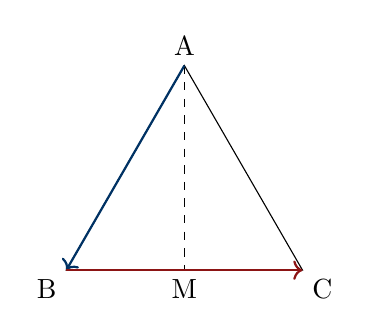
\begin{tikzpicture}[scale=1.5]
            \coordinate (A) at (0, {sqrt(3)});
            \coordinate (B) at (-1, 0);
            \coordinate (C) at (1, 0);
            \coordinate (M) at (0, 0);
            
            \draw (A)--(B)--(C)--cycle;
            \draw[dashed] (A)--(M);
            \node[above] at (A) {A};
            \node[below left] at (B) {B};
            \node[below right] at (C) {C};
            \node[below] at (M) {M};
            
            % Hint for (2)
            \draw[->, thick, printBlue] (A)--(B);
            \draw[->, thick, printRed] (B)--(C);
            
            % Parallel shift hint
            % \draw[->, dashed, printBlue!50] (B) -- ++(-0.5, {-0.5*sqrt(3)}) node[below] {$\vec{v}$};
            % \node[left, scale=0.8, gray] at (-1.2, -0.5) {始点をBにそろえる};
        \end{tikzpicture}
        \end{center}
        \vspace{8cm}
    \end{eg}
\end{any}

%-----------------------------------------------------------------------------
% 右カラム:解答スペース
%-----------------------------------------------------------------------------
\columnbreak

\begin{eg}{3 (成分計算への布石)}
    直角二等辺三角形ABC ($C=90^\circ, AC=BC=1$) において, 
    $\overrightarrow{\text{AB}} \cdot \overrightarrow{\text{AC}}$ を求めよ.
    
    \tcblower
    \vspace{12cm}
\end{eg}

\end{multicols}

%=============================================================================
% 3枚目:確認テスト(問題)
%=============================================================================
\newpage
\fancyhead[L]{\small \textcolor{black!90}{数学C $>$ 第1章--平面ベクトル $>$ 第4回--\textbf{確認テスト}}}
\begin{multicols}{2}

\begin{any}{確認テスト (A: 基本)}
    \begin{prac}{A1 (計算)}
        次のベクトル $\vec{a}, \vec{b}$ の内積を求めよ.
        \begin{enumerate}
            \item $|\vec{a}|=5, |\vec{b}|=2$, なす角 $60^\circ$
            \item $|\vec{a}|=4, |\vec{b}|=3$, なす角 $150^\circ$
            \item $|\vec{a}|=2, |\vec{b}|=5$, $\vec{a} \perp \vec{b}$
        \end{enumerate}
    \end{prac}
    \begin{answer}[height=5cm]
    \end{answer}

    \begin{prac}{A2 (大きさの計算)}
        $|\vec{a}|=2, |\vec{b}|=3, \vec{a}\cdot\vec{b}=4$ のとき, 
        なす角 $\theta$ を求めよ.
    \end{prac}
    \begin{answer}[height=5cm]
    \end{answer}
\end{any}

\columnbreak

\begin{any}{確認テスト (B: 標準)}
    \begin{prac}{B1 (正六角形の内積)}
        1辺の長さが $1$ の正六角形ABCDEFにおいて, 次の内積を求めよ.
        \begin{enumerate}
            \item $\overrightarrow{\text{AB}} \cdot \overrightarrow{\text{AF}}$
            \item $\overrightarrow{\text{AB}} \cdot \overrightarrow{\text{BC}}$
            \item $\overrightarrow{\text{AD}} \cdot \overrightarrow{\text{AF}}$
            \item $\overrightarrow{\text{AD}} \cdot \overrightarrow{\text{BE}}$
        \end{enumerate}
        
        \begin{center}
        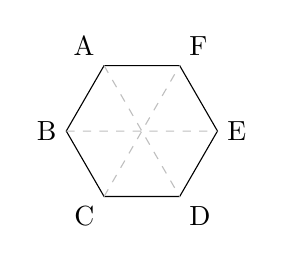
\begin{tikzpicture}[scale=0.8]
            \coordinate (O) at (0,0);
            \foreach \i in {0,60,120,180,240,300} {
                \coordinate (P\i) at (\i:1.2);
            }
            \coordinate (A) at (P120);
            \coordinate (B) at (P180);
            \coordinate (C) at (P240);
            \coordinate (D) at (P300);
            \coordinate (E) at (P0);
            \coordinate (F) at (P60);
            
            \draw (A)--(B)--(C)--(D)--(E)--(F)--cycle;
            \draw[dashed, gray!50] (A)--(D) (B)--(E) (C)--(F);
            
            \node[above left] at (A) {A}; \node[left] at (B) {B}; \node[below left] at (C) {C};
            \node[below right] at (D) {D}; \node[right] at (E) {E}; \node[above right] at (F) {F};
        \end{tikzpicture}
        \end{center}
    \end{prac}
    
    \begin{answer}[height=10cm]
    \end{answer}
\end{any}

\end{multicols}

%=============================================================================
% 4枚目:確認テスト(解答)
%=============================================================================
\newpage
\fancyhead[L]{\small \textcolor{black!90}{数学C $>$ 第1章--平面ベクトル $>$ 第4回 \textbf{【解答解説】}}}

\begin{multicols}{2}

\begin{any}{解答 (A: 基本)}
    \begin{prac}{A1 (計算)}
        (1) $5 \times 2 \times \cos 60^\circ = 10 \times \frac{1}{2} = \boldsymbol{5}$ \\
        (2) $4 \times 3 \times \cos 150^\circ = 12 \times (-\frac{\sqrt{3}}{2}) = \boldsymbol{-6\sqrt{3}}$ \\
        (3) 垂直ならば内積は $\boldsymbol{0}$
    \end{prac}

    \begin{answer}[height=5cm]
    \color{printRed}
    \textbf{A2 解答:} \\
    定義より $\vec{a} \cdot \vec{b} = |\vec{a}| |\vec{b}| \cos\theta$.
    値を代入すると,
    \[ 4 = 2 \times 3 \times \cos\theta \]
    \[ 6\cos\theta = 4 \implies \cos\theta = \frac{2}{3} \]
    よって $\boldsymbol{\cos\theta = \frac{2}{3}}$ \\
    (具体的な角度が出ない場合は $\cos$ の値で答える)
    \end{answer}
\end{any}

\columnbreak

\begin{any}{解答 (B: 標準)}
    \begin{answer}[height fill]
    \color{printRed}
    \textbf{B1 解答:} \\
    1辺の長さは1. 内角は$120^\circ$.
    
    (1) $\overrightarrow{\text{AB}} \cdot \overrightarrow{\text{AF}}$ \\
    始点はAで揃っている. なす角は $\angle BAF = 120^\circ$. \\
    $1 \times 1 \times \cos 120^\circ = 1 \cdot (-\frac{1}{2}) = \boldsymbol{-\frac{1}{2}}$
    
    (2) $\overrightarrow{\text{AB}} \cdot \overrightarrow{\text{BC}}$ \\
    始点が異なる. $\overrightarrow{\text{AB}}$ を平行移動して, 始点をBに合わせる(BからAの逆へ伸ばす). \\
    なす角は $180^\circ - \angle ABC = 180^\circ - 120^\circ = 60^\circ$. \\
    $1 \times 1 \times \cos 60^\circ = \boldsymbol{\frac{1}{2}}$
    
    (3) $\overrightarrow{\text{AD}} \cdot \overrightarrow{\text{AF}}$ \\
    ADは外接円の直径で長さ2. $\angle DAF = 60^\circ$. \\
    $2 \times 1 \times \cos 60^\circ = 2 \cdot \frac{1}{2} = \boldsymbol{1}$
    
    (4) $\overrightarrow{\text{AD}} \cdot \overrightarrow{\text{BE}}$ \\
    $\overrightarrow{\text{BE}}$ と $\overrightarrow{\text{AD}}$ は平行ではない...? いや, BEも対角線. \\
    図を見ると $\overrightarrow{\text{AD}}$ と $\overrightarrow{\text{BE}}$ のなす角は $60^\circ$.
    長さは共に $2$. \\
    $2 \times 2 \times \cos 60^\circ = 4 \cdot \frac{1}{2} = \boldsymbol{2}$
    \end{answer}
\end{any}

\end{multicols}
\end{document}